\documentclass[./dissertation.tex]{subfiles}
\usepackage{algorithm2e}
\begin{document}

    \contentchapter{Methodology}
    We look to discover the potential of applying components of the VAE methodology to DML systems. We test this through presenting incremental modifications to the basic DML architecture. Each modified architecture corresponds to a claim about how a specific part of the VAE training regime and loss function may be adapted to assist the performance of a DML method for a semi-supervised dataset.
    
    \RestyleAlgo{ruled}
    \SetKwComment{Comment}{/* }{ */}

    \begin{algorithm}
    \caption{Base DML Training Routine}\label{alg:two}
    \KwIn{Dataset dataset $D$, encoder network $f$, metric loss function $m$, learning rate $\gamma$}
    \KwResult{trained encoder $f$}
    \For{batch $x$, $y$ in $D$}{
        $z = f(x)$\;
        $c = m(z, y)$\;
        Calculate gradients given cost function\;
        Apply Gradients to f\;
    }
    \end{algorithm}
     
    \section{Claim 1: Benefits of Reconstruction Loss}
    We first look to evaluate the claim that adding a reconstruction loss to a DML system can improve the quality of clustering in the latent representations on a semi-supervised dataset. Reconstruction loss in and of itself enforces a similar semantic mapping onto the latent space as a metric loss, but can be computed  without labelled data. In theory, we believe that the added constraint that the latent vector must be reconstructed to approximate the original output will train the spatial positioning to reflect semantic information. Following this reasoning, with observations which share similar semantic information, specifically observations of the same class, should intuitively be positioned nearby within the latent space. To test if this intuition occurs in practice, we evaluate if a DML model with an autoencoder structure and reconstruction loss (described in further detail below) will perform better than a plain DML model in terms of clustering quality. This will be especially evident in semi-supervised datasets when the amount of labelled data is not feasible for solely supervised DML. \\
    
    Given a semi-supervised dataset, we assume a standard DML system will use only the labelled data and train given a metric loss $L_{metric}$. Our modified model will extend the DML system's training regime by adding a decoder network which takes the latent point $z$ as input and produces an output $\hat{x}$. The loss function is then modified such that there is a supervised loss $L_{S}$ which is identical to the metric loss $L_{metric}$ and an unsupervised loss that is identical to the reconstruction loss $L_{U}$. Each epoch, the total loss alternates between the supervised and unsupervised loss, such $L = (1 - \alpha) L_{S} + \alpha L_{U}$ on odd number epochs and $L = \alpha L_{U}$ for even number epochs. $\alpha$ is a hyperparameter which modulates the impact of the reconstruction loss on total loss for the DML autoencoder. The unsupervised loss is computed in both the supervised and unsupervised stages because of a software constraint which requires each parameter to be used in the loss computation for every epoch.  \\

    \begin{algorithm}
    \caption{DML Autoencoder Training Routine}\label{alg:two}
    \KwIn{Dataset dataset $D$, encoder network $f$, decoder network $g$, metric loss function $m$, learning rate $\gamma$, coefficient $\alpha$}
    \KwResult{trained encoder $f$}
    \For{batch $x$, $y$ in $D$}{
        $z = f(x)$\;
        $\hat{x} = g(z)$\;
        \eIf{s} {
            $c = (1 - \alpha) * m(z, y) + \alpha * MSE(\hat{x}, x)$\;
        }
        {
            $c = \alpha * MSE(\hat{x}, x)$\;
        }
        Calculate gradients given cost function\;
        Apply Gradients to f\;
    }
    \end{algorithm}    
    
    \section{Claim 2: Incorporating Inductive Bias with Prior}
    Say we are aware that a dataset has $n$ classes. It may be useful to encourage that there are $n$ clusters in the latent space of a DML model. This can be enforced by using a prior distribution containing $n$ many Gaussians. As we wish to measure only the affect of inducing bias on the representation without adding any complexity to the model, the prior distribution will not be learnable (unlike VAE with VampPrior). By testing whether the classes of points in the latent space are organized along the prior components we can test whether bias can be induced using a prior to constrain the latent space of a DML. By testing whether clustering improves performance, we can evaluate whether this inductive bias is helpful. \\
    
    Given a fully supervised dataset, we assume a standard DML system will use only the labelled data and train given a metric loss $L_{metric}$. Our modified model will extend the DML system's training regime by adding a KL divergence term to the loss which measures the difference between posterior distributions and a prior distribution. It should also be noted that, like the VAE encoder, we will map the input not to a latent point but to a latent distribution. The latent point is stochastically sampled from the latent distribution during training. Mapping the input to a distribution instead of a point will allow us to calculate the KL divergence. \\
    
    The loss function is then modified such that the total loss $L$ is equal to a weighted sum between the metric loss term $L_{metric}$ and the KL divergence term $L_{KL}$. As is true in the previous section, the total loss alternates between the supervised and unsupervised loss, such $L = (1 - \alpha) L_{S} + \alpha L_{U}$ on odd number epochs and $L = \alpha L_{U}$ for even number epochs.
    
    In practice, we will be evaluating a DML model with a unit prior and a DML model with a mixture of gaussians (GMM) prior. The latter model constructs the prior as a mixture of $n$ gaussians -- each the vertice of the unit (i.e. each side is 2 units long) hypercube in the latent space. The standard deviation of each component is equal to one-third of the distance between components. Constructing the prior in this way is beneficial in that it is ensured that each component is evenly spaced within the latent space, but is limiting in that there must be exactly $2^{d}$ components in the GMM prior. Thus, to test, we will limit a dataset to 8 classes and test with the latent space dimensionality of 2, such that there are $2^{3}=8$ gaussian components in the prior and 8 classes. The drawback of this decision is that the manifold of the chosen dataset may not necessarily exist in 3 dimensions. Choosing gaussian components from a d-dimensional hypersphere in the latent space $\mathcal{R}^{d}$ would solve this issue, but there does not appear to be a solution for choosing $n$ evenly spaced points spanning $d$ dimensions on a d-dimensional hypersphere. KL Divergence is calculated with a monte carlo approximation for the GMM and analytically with the unit prior.
    
    \begin{algorithm}
    \caption{DML with Prior Training Routine}\label{alg:two}
    \KwIn{Dataset dataset $D$, encoder network $f$, metric loss function $m$, learning rate $\gamma$, coefficient $\alpha$, prior distribution mean and log-variance $\mu_{p}$, $\sigma_{p}$}
    \KwResult{trained encoder $f$}
    \For{batch $x$, $y$ in $D$}{
        $\mu, \sigma = f(x)$\;
        $z \sim N(\mu, \sigma)$\;
        \eIf{s} {
            $c = (1 - \alpha) * m(z, y) + \alpha * KL(z, \mu, \sigma, \mu_{p}, \sigma_{p})$\;
        }
        {
            $c = \alpha * KL(z, \mu, \sigma, \mu_{p}, \sigma_{p})$\;
        }
        Calculate gradients given cost function\;
        Apply Gradients to f\;
    }
    \end{algorithm}
    \begin{algorithm}
    \caption{Monte-Carlo KL Divergence Algorithm}\label{alg:two}
    \KwIn{Latent variable $z$, approximate posterior distribution mean and variance $\mu$,$\sigma$, prior distribution mean and log-variance $\mu_{p}$, $\sigma_{p}$}
    \KwResult{KL Divergence between distributions $q$ and $p$}
    $P(z|\mu, \sigma) = -0.5 * \frac{(z - \mu)^{2}}{\exp{\sigma}}$\;
    $Q(z|\mu_{p}, \sigma_{p}) = -0.5 * \frac{(z - \mu_{p})^{2}}{\exp{\sigma_{p}}}$\;
    \Return $Q(z|\mu_{p}, \sigma_{p}) - P(z|\mu, \sigma)$
    \end{algorithm}
    
    \section{Claim 3: Jointly Optimizing DML with VAE}
    The third claim we look to evaluate is that given a semi-supervised dataset, optimizing a DML model jointly with a VAE on the VAE’s latent space will produce superior clustering than the DML model or VAE individually. The intuition behind this approach is that DML methods can learn from only supervised data and VAE methods can learn from only unsupervised data; the proposed methodology will optimize both tasks simultaneously to learn from both supervised and unsupervised data. This approach has been previously tested: *take from related lit*. We look to provide a granular experiment across several datasets and both contrastive and non-contrastive metric losses to provide for the experiment.  \\
    
    The MetricVAE implementation we create jointly optimizes the VAE task and DML task on the VAE latent space. Across epochs, the MetricVAE model alternates between training only the unsupervised task $L_{U}$ and the semi-supervised task $\alpha * L_{U} + (1 - \alpha) * L_{S}$. $\alpha$ is a hyperparameter which dictates the percentage the unsupervised loss is weighted against the supervised loss in the semi-supervised stage. The software tool used (Pytorch Lightning) used to construct the models restricts not using all parameters in the computation of the loss for a given epoch; thus we have a semi-supervised stage consisting of the unsupervised and the supervised loss instead of solely a supervised stage, as the the supervised loss does not make use of the parameters in the decoder. 
    
    \begin{algorithm}
    \caption{DML VAE Training Routine}\label{alg:two}
    \KwIn{Dataset dataset $D$, encoder network $f$, decoder network $g$, metric loss function $m$, learning rate $\gamma$, coefficient $\alpha$, coefficient $\beta$, prior distribution mean and log-variance $\mu_{p}$, $\sigma_{p}$}
    \KwResult{trained encoder $f$}
    \For{batch $x$, $y$ in $D$}{
        $\mu, \sigma = f(x)$\;
        $z \sim N(\mu, \sigma)$\;
        $\hat{x} = g(z)$\;
        $c_{vae} = MSE(x, x_{hat}) + \beta * KL(z, \mu, \sigma, \mu_{p}$\;
        \eIf{s} {
            $c = (1 - \alpha) * m(z, y) + \alpha * c_{vae}$\;
        }
        {
            $c = \alpha * c_{vae}$\;
        }
        Calculate gradients given cost function\;
        Apply Gradients to f\;
    }
    \end{algorithm}

    \begin{figure}[h]
        \centering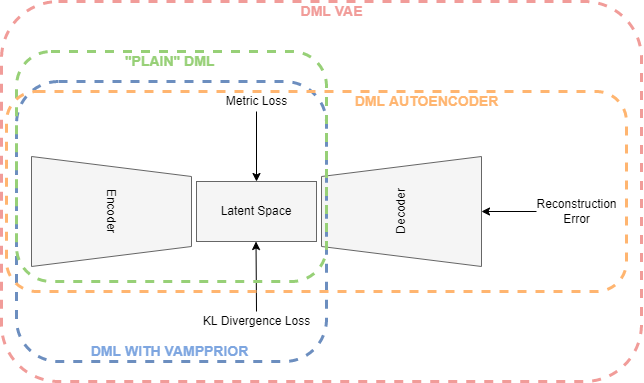
\includegraphics[width=0.5\textwidth]{figures/DML_Arcs.drawio.png}
        \caption{Comparison of Modified DML Architectures Presented}
        \label{Triplet Loss Diagram}
    \end{figure}

    
\end{document}
